\documentclass[runningheads]{llncs}
\usepackage[T1]{fontenc}
\usepackage{amsmath,amssymb,booktabs,graphicx,multirow}
\usepackage{tikz}
\usetikzlibrary{arrows.meta,shapes.geometric,decorations.pathreplacing,calc,shadows}
\usepackage[hidelinks]{hyperref}
\setlength{\emergencystretch}{1.5em}
\newcommand{\Hpost}{H_{\mathrm{post}}}
\newcommand{\Hpre}{H_{\mathrm{pre}}}
\begin{document}
\title{How Much of the Oracle Gap Is Headroom? Test Reuse and Outcome Luck in Evaluating Label Acquisition}
\titlerunning{How Much of the Oracle Gap Is Headroom?}
\author{Anonymous Authors}
\authorrunning{Anonymous Authors}
\institute{Anonymous Institution}
\maketitle

\begin{abstract}
Active-learning benchmarks measure headroom with oracles that choose labels after seeing them. Part of an oracle's lead is unattainable by any strategy: it comes from reusing the evaluation set and, when outcomes are random, from luck in the acquired labels. We split the benchmark oracle gap into test reuse, a residual that is the benchmark analogue of the value of perfect information about the acquired labels, and the gain of a held-out ex-ante selector, and we bracket the residual between plug-in and cross-fitted estimates. Across eight credit, readmission, marketing, e-mail and digit cohorts, the residual's share of the gap rises with label noise (Spearman $0.81$ and $0.88$ at the two ends of the bracket; 3/3 cohorts under injected label flips), from 10--16\% on digits and spam to 50--60\% on noisy credit outcomes. Exhaustive search in pools of up to 20 candidates, stronger ex-ante search and five outcome models leave these findings unchanged. In a benchmark-style setting, every practical strategy falls materially short of the reported oracle up to 256 labels; once reuse and luck are removed, a minority does at 256 labels and none at 512. Reported oracle gaps should be corrected before they are read as headroom.
\keywords{Active learning \and Evaluation \and Oracle bounds \and Aleatoric uncertainty \and Value of information}
\end{abstract}

% ======================================================================
\section{Introduction}
\label{sec:intro}
How much better could a label-acquisition strategy be? Active-learning research increasingly answers with an \emph{oracle}: a selector that, unlike any deployable strategy, may look at the labels it acquires and at the evaluation data, and so traces the best attainable learning curve. Recent benchmarks build greedy oracles that add, step by step, the candidate whose \emph{realized} label most improves test performance~\cite{werner2023comparable,werner2024cdalbench}, and best-of-strategies oracles that pick, per batch, the strategy whose labeled batch helps most~\cite{huseljic2026boss}. The distance between oracle and practical strategies is then read as headroom; state-of-the-art strategies are reported to ``fall noticeably short of oracle performance''~\cite{huseljic2026boss}. This is part of a broader effort to make active-learning evaluation reliable~\cite{luth2023navigating,ji2023randomness}.

An oracle that selects with realized labels is an \emph{ex-post} benchmark, and part of its advantage is unreachable by construction. Werner et al.\ note that their oracle overfits the test set~\cite{werner2023comparable}. Outcome luck in the training labels is a second, separate source: if an applicant's repayment, a patient's readmission or a customer's response is random given the covariates, then among all label sets a strategy could have bought some will turn out well, and only an observer of the outcomes can pick that one. Splitting the test set does not remove it. The distinction between ex-ante and ex-post regret is familiar in decision-focused learning~\cite{schutte2023robust}, and in bandits expected regret exceeds pseudo-regret by a noise-driven term~\cite{bubeck2012regret,audibert2010regret}. What is missing for label acquisition is a way to \emph{measure} both sources on real data, and evidence of whether they change what benchmarks conclude.

We make three contributions, graded by the kind of evidence behind them.
\begin{itemize}
\item \textbf{An accounting with bounds} (Section~\ref{sec:protocol}). The benchmark oracle's lead splits into test reuse, a residual and the gain of a cross-fitted ex-ante selector. The residual is the benchmark analogue of the floor $F$, the expected value of perfect information about the acquired labels over a fixed family of feasible sets~\cite{howard1966information}; we prove distribution-free bounds on $F$ and bracket the residual between plug-in and cross-fitted estimates, whose biases have opposite signs.
\item \textbf{A validated protocol for real data} (Section~\ref{sec:validation}), using an outcome model fitted on disjoint records. It recovers known-probability values, matches recorded-outcome hindsight, agrees with exhaustive search over all feasible sets in pools of 12, 16 and 20 candidates, is insensitive to stronger ex-ante search, and keeps its conclusions under five outcome models.
\item \textbf{Findings} across eight cohorts (Sections~\ref{sec:findings}--\ref{sec:replay}). The residual's share of the oracle gap tracks label noise across cohorts, under within-cohort label-flip interventions and at later learning-curve positions. In a benchmark-style pool-based setting, the conclusion that practical strategies fall materially short of the oracle holds early in the learning curve but disappears later, where most of the reported gap is test reuse. A case study of risk-constrained acquisition with delayed labels, including our own conservative policy DC-PRISM, shows which strategies win the remaining gap.
\end{itemize}

\begin{figure}[t]
 \centering
 \resizebox{\linewidth}{!}{% =====================================================================
% Framework figure with characters (TikZ, editable). Scaled to \linewidth by \resizebox in main.tex.
% Needs: \usepackage{tikz}
%        \usetikzlibrary{arrows.meta,shapes.geometric,decorations.pathreplacing,calc,shadows}
% Colour code used throughout the paper:
%   blue = deployable (ex-ante) part, orange = aleatoric floor, gray = test-set reuse.
% Bar proportions follow the real-label row of Table 1 (12% reuse, 52% residual, 36% deployable).
% Coordinates are in cm. Characters: \person{x}{y-feet}{scale}{shirt}{hair};
% candidates: \applicant{x}{y}{size}{risk colour}. Previous version: framework_v1_no_characters.tex
% =====================================================================
\definecolor{dep}{HTML}{4C78A8}\definecolor{flo}{HTML}{F58518}\definecolor{reu}{HTML}{9D9D9D}
\definecolor{lowr}{HTML}{54A24B}\definecolor{midr}{HTML}{EECA3B}\definecolor{highr}{HTML}{E45756}
\colorlet{shirtB}{dep!80}\colorlet{shirtC}{flo!85}\colorlet{shirtD}{teal!75}\colorlet{neutral}{black!45}
\definecolor{skin}{HTML}{F2C9A0}\definecolor{hairA}{HTML}{3B2F2F}\definecolor{hairB}{HTML}{8C5A3C}\definecolor{hairC}{HTML}{2E2E3A}
\begin{tikzpicture}[
  font=\sffamily\small, >={Stealth[length=2mm]},
  panel/.style={draw=#1!55, fill=#1!6, rounded corners=6pt, line width=0.7pt},
  ptitle/.style={font=\sffamily\normalsize\bfseries, anchor=north west, text=black!85},
  step/.style={circle, fill=#1, text=white, font=\sffamily\footnotesize\bfseries, inner sep=1.4pt},
  flow/.style={->, line width=1.1pt, draw=black!55},
  thin/.style={draw=black!45, line width=0.5pt},
  card/.style={draw=black!25, fill=white, rounded corners=3pt, drop shadow={opacity=0.15, shadow xshift=0.4pt, shadow yshift=-0.4pt}},
  bubble/.style={draw=black!35, fill=white, ellipse, inner sep=1pt, drop shadow={opacity=0.12, shadow xshift=0.3pt, shadow yshift=-0.3pt}},
]
% ---------------------------------------------------------------- characters and icons
\newcommand{\person}[5]{% x, y (feet), scale, shirt colour, hair colour
  \begin{scope}[shift={(#1,#2)}, scale=#3]
    \fill[#4] (-0.40,0) .. controls (-0.42,0.50) and (-0.26,0.70) .. (0,0.70) .. controls (0.26,0.70) and (0.42,0.50) .. (0.40,0) -- cycle;
    \fill[#4!70!black] (-0.06,0.70) -- (0,0.55) -- (0.06,0.70) -- cycle;
    \fill[skin] (-0.07,0.66) rectangle (0.07,0.78);
    \fill[skin] (0,0.98) circle (0.24);
    \fill[#5] (-0.25,1.00) .. controls (-0.25,1.30) and (0.25,1.30) .. (0.25,1.00)
              .. controls (0.12,1.10) and (-0.12,1.12) .. (-0.25,1.00) -- cycle;
    \fill[black!80] (-0.08,0.97) circle (0.025); \fill[black!80] (0.08,0.97) circle (0.025);
    \draw[black!60, line width=0.35pt] (-0.06,0.88) .. controls (-0.02,0.85) and (0.02,0.85) .. (0.06,0.88);
  \end{scope}}
\newcommand{\applicant}[4]{% x, y, size r, colour : small person icon (applicant)
  \fill[#4, opacity=0.9] ($(#1,#2)+(-#3,-1.05*#3)$) arc (180:0:#3 and 0.85*#3) -- cycle;
  \fill[#4!80!black] ($(#1,#2)+(0,0.25*#3)$) circle (0.52*#3);}
\newcommand{\die}[3]{% x, y, size
  \draw[card] (#1,#2) rectangle ++(#3,#3);
  \foreach \dx/\dy in {0.25/0.25,0.75/0.25,0.5/0.5,0.25/0.75,0.75/0.75}
    \fill[black!70] ($(#1,#2)+(\dx*#3,\dy*#3)$) circle (0.045*#3/0.35);}
\newcommand{\padlock}[3]{% x, y, size
  \draw[white, line width=1.3pt] ($(#1,#2)+(-0.26*#3,0.28*#3)$) -- ++(0,0.22*#3) arc (180:0:0.26*#3) -- ++(0,-0.22*#3);
  \fill[white, rounded corners=1pt] ($(#1,#2)+(-0.42*#3,-0.30*#3)$) rectangle ($(#1,#2)+(0.42*#3,0.30*#3)$);
  \fill[flo] ($(#1,#2)+(0,0.04*#3)$) circle (0.08*#3);}

% ================================================================ PANEL 1: acquisition
\draw[panel=gray] (0,0) rectangle (4.2,5.6);
\node[step=black!70] at (0.32,5.28) {1};
\node[ptitle] at (0.55,5.48) {Acquire under risk};
\foreach \x/\y/\r/\c in {1.55/4.45/0.13/lowr, 2.05/4.65/0.15/lowr, 2.55/4.40/0.11/lowr, 3.05/4.70/0.18/midr, 3.60/4.35/0.20/highr,
                         1.70/3.80/0.17/midr, 2.25/3.95/0.12/lowr, 2.80/3.75/0.13/lowr, 3.35/3.85/0.22/highr,
                         1.60/3.10/0.12/lowr, 2.15/3.20/0.19/highr, 2.70/3.05/0.13/midr, 3.25/3.15/0.12/lowr, 3.75/3.30/0.16/midr}
  {\applicant{\x}{\y}{\r}{\c}}
\draw[dashed, line width=0.9pt, draw=dep, rounded corners=8pt] (1.25,4.05) -- (1.28,4.95) -- (2.85,5.00) -- (3.05,4.18) -- (3.05,3.50) -- (2.45,3.40) -- (1.32,3.48) -- cycle;
\node[font=\sffamily\footnotesize, text=dep, anchor=west] at (1.10,2.62) {feasible: $R_\alpha(S)\le B$};
\person{0.62}{0.95}{1.05}{dep}{hairA}
\draw[card] (0.98,1.25) rectangle (1.32,1.70); \foreach \yy in {1.36,1.46,1.56} {\draw[black!40] (1.04,\yy) -- (1.26,\yy);}
\node[font=\sffamily\footnotesize, text=black!70, align=left, anchor=west] at (1.45,1.62) {lender buys labels\\ by approving};
\applicant{1.25}{0.66}{0.09}{lowr}\applicant{1.50}{0.66}{0.09}{midr}\applicant{1.75}{0.66}{0.09}{highr}
\node[anchor=west, font=\sffamily\footnotesize, text=black!65] at (1.86,0.66) {risk};
\applicant{2.62}{0.66}{0.07}{neutral}\applicant{2.88}{0.66}{0.13}{neutral}
\node[anchor=west, font=\sffamily\footnotesize, text=black!65] at (3.02,0.66) {size};
\node[font=\sffamily\footnotesize, text=black!55] at (2.10,0.24) {history $+$ pending $+$ pool};

% ================================================================ PANEL 2: two oracles
\draw[panel=violet] (4.65,0) rectangle (9.75,5.6);
\node[step=black!70] at (4.97,5.28) {2};
\node[ptitle] at (5.20,5.48) {Two oracles};
\person{5.45}{3.05}{0.95}{shirtB}{hairB}
\node[anchor=west, font=\sffamily\small\bfseries, text=dep] at (5.00,2.72) {ex-ante};
\node[bubble, minimum width=3.15cm, minimum height=1.55cm] (tb) at (7.75,3.95) {};
\fill[white, draw=black!35] (6.20,3.55) circle (0.07); \fill[white, draw=black!35] (6.02,3.40) circle (0.045);
\die{6.65}{3.70}{0.30}\die{6.95}{3.95}{0.30}\die{6.95}{3.47}{0.30}
\draw[->, black!55, line width=0.8pt] (7.35,3.88) -- (7.62,3.88);
\foreach \i/\h in {0/0.62,1/0.38,2/0.52,3/0.70} {\fill[dep!75] (7.75+\i*0.27,3.45) rectangle ++(0.18,\h);}
\draw[line width=1pt, dep] (7.98,3.38) -- (8.20,3.38);
\node[font=\sffamily\footnotesize, text=black!70, align=left, anchor=west] at (6.45,2.68) {best by \emph{expected} loss\\ over label replicates};
\draw[violet!30, line width=0.6pt] (4.85,2.32) -- (9.55,2.32);
\person{5.45}{0.45}{0.95}{shirtC}{hairC}
\node[anchor=west, font=\sffamily\small\bfseries, text=flo] at (5.00,0.18) {ex-post};
\fill[flo!35] (6.55,0.40) -- (7.25,0.40) -- (7.10,0.62) -- (6.70,0.62) -- cycle;
\shade[inner color=white, outer color=violet!40] (6.90,1.15) circle (0.50); \draw[violet!60] (6.90,1.15) circle (0.50);
\node[text=lowr!80!black, font=\small] at (6.75,1.25) {$\checkmark$};
\node[text=highr, font=\small] at (7.05,1.02) {$\times$};
\draw[flo, line width=0.8pt, dashed, ->] (5.95,1.45) .. controls (6.15,1.70) and (6.30,1.65) .. (6.42,1.45);
\node[font=\sffamily\footnotesize, text=black!70, align=left, anchor=west] at (7.50,1.20) {best after\\ seeing the\\ \emph{realized} labels};

% ================================================================ PANEL 3: decomposition
\draw[panel=orange] (10.20,0) rectangle (13.50,5.6);
\node[step=black!70] at (10.52,5.28) {3};
\node[ptitle] at (10.75,5.48) {Split the gap};
\def\bx{10.50}\def\bw{0.62}
\fill[reu] (\bx,0.55) rectangle ++(\bw,0.50);
\fill[flo] (\bx,1.05) rectangle ++(\bw,2.15);
\fill[dep] (\bx,3.20) rectangle ++(\bw,1.48);
\draw[white, line width=1pt] (\bx,1.05) -- ++(\bw,0) (\bx,3.20) -- ++(\bw,0);
\padlock{\bx+0.31}{2.12}{0.46}
\node[font=\sffamily\scriptsize\bfseries, text=black!75] at (\bx+0.31,4.84) {reported};
\draw[decorate, decoration={brace, amplitude=4pt}, thin] (\bx+\bw+0.08,4.66) -- (\bx+\bw+0.08,3.22);
\draw[decorate, decoration={brace, amplitude=4pt}, thin] (\bx+\bw+0.08,3.18) -- (\bx+\bw+0.08,1.07);
\draw[decorate, decoration={brace, amplitude=3pt}, thin] (\bx+\bw+0.08,1.03) -- (\bx+\bw+0.08,0.57);
\node[anchor=west, align=left, font=\sffamily\footnotesize] at (\bx+\bw+0.25,3.94) {\textbf{\textcolor{dep}{deployable}}\\ \textbf{\textcolor{dep}{gap}}\\ (gainable)};
\node[anchor=west, align=left, font=\sffamily\footnotesize] at (\bx+\bw+0.25,2.12) {\textbf{\textcolor{flo}{residual}}\\ (luck in\\ the labels)};
\node[anchor=west, align=left, font=\sffamily\footnotesize] at (\bx+\bw+0.25,0.80) {\textbf{\textcolor{black!60}{test reuse}}};

% ================================================================ PANEL 4: predict and act
\draw[panel=teal] (13.95,0) rectangle (18.10,5.6);
\node[step=black!70] at (14.27,5.28) {4};
\node[ptitle] at (14.50,5.48) {Audit and act};
\draw[->, thin] (15.35,3.05) -- (17.80,3.05) node[above left, font=\sffamily\footnotesize, text=black!65, xshift=2pt, yshift=1pt] {noise};
\draw[->, thin] (15.35,3.05) -- (15.35,4.85) node[right, font=\sffamily\footnotesize, text=black!65, xshift=1pt, yshift=-4pt] {residual share};
\draw[flo, line width=1.2pt] plot[smooth, tension=0.6] coordinates {(15.50,3.25) (16.05,3.40) (16.60,3.85) (17.15,4.30) (17.60,4.55)};
\foreach \x/\y in {15.60/3.22,16.10/3.48,16.50/3.75,16.85/4.15,17.20/4.25,17.50/4.60} {\fill[flo!80!black] (\x,\y) circle (0.05);}
\person{14.55}{2.95}{0.85}{shirtD}{hairB}
\draw[black!70, line width=1.4pt] (14.92,3.72) -- (15.06,3.88);
\draw[black!70, line width=1pt, fill=white, fill opacity=0.6] (15.18,4.02) circle (0.18);
\node[font=\footnotesize, text=black!80, align=center] at (16.10,2.20) {$F_{\mathrm{lo}}\le F\le F_{\mathrm{up}}$\\[1pt]
  \scriptsize distribution-free bounds};
\begin{scope}[shift={(16.05,1.12)}]
  \fill[dep!25, opacity=0.9] (-0.50,0) circle (0.62); \fill[lowr!30, opacity=0.9] (0.50,0) circle (0.62);
  \draw[dep, line width=0.8pt] (-0.50,0) circle (0.62); \draw[lowr!80!black, line width=0.8pt] (0.50,0) circle (0.62);
  \node[font=\sffamily\footnotesize, text=dep!80!black] at (-0.60,0) {proxy};
  \node[font=\sffamily\footnotesize, text=lowr!50!black] at (0.58,0) {learner};
\end{scope}
\node[font=\sffamily\footnotesize, text=black!70] at (16.05,0.28) {match $\Rightarrow$ gap closed};

% ================================================================ flows between panels
\draw[flow] (4.20,2.80) -- (4.65,2.80);
\draw[flow, draw=dep]  (9.75,3.95) -- (10.20,3.95);
\draw[flow, draw=flo]  (9.75,1.20) -- (10.20,1.20);
\draw[flow] (13.50,2.80) -- (13.95,2.80);

% ================================================================ bottom strip: estimation on real data
\draw[panel=gray] (0,-1.75) rectangle (18.10,-0.40);
\node[font=\sffamily\small\bfseries, anchor=west, text=black!80] at (0.20,-1.07) {Estimation on real data};
\node[cylinder, shape border rotate=90, aspect=0.25, draw=black!55, fill=white, minimum height=0.85cm, minimum width=0.62cm] (db) at (4.45,-1.07) {};
\foreach \yy in {-1.25,-1.08,-0.91} {\draw[black!30] (4.17,\yy) -- (4.73,\yy);}
\node[anchor=west, font=\sffamily\footnotesize, align=left] at (4.80,-1.07) {disjoint\\ records};
\draw[flow] (6.05,-1.07) -- (6.40,-1.07);
\node[card, font=\sffamily\footnotesize, inner sep=3pt] at (7.35,-1.07) {$\hat p$ (boosting)};
\draw[flow] (8.32,-1.07) -- (8.62,-1.07);
\die{8.72}{-1.27}{0.38}\die{9.18}{-1.27}{0.38}
\node[anchor=west, font=\sffamily\footnotesize, align=left] at (9.70,-1.07) {label replicates $Y^{(r)}$\\ feed both oracles};
\node[anchor=west, font=\sffamily\footnotesize, text=lowr!70!black] at (13.55,-0.85) {$\checkmark$ recovers known-$p$ values};
\node[anchor=west, font=\sffamily\footnotesize, text=lowr!70!black] at (13.55,-1.30) {$\checkmark$ greedy $\approx$ exact search};
\draw[->, dashed, draw=black!45, line width=0.8pt] (7.35,-0.40) -- (7.35,-0.05);
\end{tikzpicture}
}
 \caption{Overview. (1) A lender buys labels by approving applicants, under a risk budget. (2) The ex-ante oracle picks the set with the best \emph{expected} loss over outcome replicates; the ex-post oracle picks after seeing the \emph{realized} labels. (3) The reported oracle gap splits into test reuse, the residual (luck in the labels) and a deployable part. (4) Bounds and noise diagnostics audit the residual; whether a strategy closes the deployable part depends on whether its information proxy matches the learner. Bottom: an outcome model $\hat p$ fitted on disjoint records generates label replicates for both oracles.}
 \label{fig:framework}
\end{figure}

% ======================================================================
\section{Setting}
\label{sec:setting}
At round $t$ a learner holds a labeled history $D_t$, the covariates of pending acquisitions $O_t$ (selected but not yet resolved), an unlabeled candidate pool $C_t$ and target covariates $Q_t$. Candidate $i$ has a binary outcome $Y_i$, revealed only after acquisition, and a visible exposure $e_i\ge0$. A strategy chooses $S_t\subseteq C_t$ from the visible information $\mathcal H_t$. Learning is measured by the Brier score~\cite{brier1950verification} of a downstream learner (an $\ell_2$-logistic model, gradient boosting or a one-hidden-layer network); $L(S;Y)$ is its test loss after fitting on $D\cup O\cup S$, where $Y$ collects the hidden training outcomes of $O$ and $S$.

\paragraph{Risk budget.} In our main application, acquiring a label is an action with exposure: a lender observes repayment only by approving an applicant~\cite{lakkaraju2017selective,wei2021selective}, and labels of earlier approvals are still pending. With a risk score $q_i$, $\ell=\log(1/\alpha)$ and $\phi(q)=q(1-q)$ for $q\le\frac12$ ($\frac14$ otherwise), a set is feasible if
\begin{equation}
 R_\alpha(S)=\sum_{i\in S}e_iq_i+\Big(2\ell\sum_{i\in S}e_i^2\phi(q_i)\Big)^{1/2}+\frac{\ell}{3}\max_{i\in S}e_i\le B_t .
 \label{eq:envelope}
\end{equation}
This is a sub-gamma tail bound~\cite{boucheron2013concentration}: if outcomes are conditionally independent and $p_i\le q_i$, realized adverse exposure exceeds $R_\alpha(S)$ with probability at most $\alpha=0.1$. Our scores (a Wilson-shifted~\cite{wilson1927probable} upper quantile of 40 Laplace draws of the fitted logit) do not guarantee $p_i\le q_i$, so we treat~\eqref{eq:envelope} as an \emph{operational} budget shared by all strategies. $B_t$ is $1.03$ times the envelope of the $k=6$ lowest-risk candidates. The \emph{quantity reference} $M_K$ is the largest feasible set, found by enumeration for up to 16 candidates and otherwise by an exposure-stratified search whose cardinality we certified exactly in all 1{,}408 states where we checked it. For cohorts without a natural exposure, $e_i=1$. With a constant score $q_i\equiv\frac12$ and $e_i=1$ the envelope depends on $|S|$ only and the budget admits exactly six labels: the usual cardinality budget of pool-based benchmarks, which we use in Section~\ref{sec:bench}.

% ======================================================================
\section{Decomposing the Oracle Gap}
\label{sec:protocol}
\paragraph{Family oracles and the floor.} Fix the visible information $\mathcal H$ and a finite family $\mathcal F$ of feasible sets, constructed from $\mathcal H$ only and containing $M=M_K$. Let $\bar L(S;Y)$ be the test loss with test-label noise integrated out, and write the gain of $S$ over the reference as $d_S=\bar L(M;Y)-\bar L(S;Y)$, with mean $\mu_S=\mathbb E[d_S\mid\mathcal H]$. Two oracles are natural:
\begin{equation}
 \Hpost=\mathbb E\big[\max_{S\in\mathcal F}d_S\mid\mathcal H\big],\qquad
 \Hpre=\max_{S\in\mathcal F}\mu_S .
\end{equation}
$\Hpost$ is the lead of an oracle that chooses after seeing the hidden training labels; $\Hpre$ is the lead of the best choice that does not see them. Their difference
\begin{equation}
 F=\Hpost-\Hpre\ \ge 0
\end{equation}
is the \emph{floor}: the expected value of perfect information about the training outcomes~\cite{howard1966information,raiffa1961applied}. No strategy that chooses from $\mathcal F$ on the basis of $\mathcal H$ can attain it, since such a strategy's expected gain $\Gamma_\pi$ is at most $\Hpre$; hence $\Hpost-\Gamma_\pi = F+(\Hpre-\Gamma_\pi)$, and only the second term, the \emph{selection gap}, is open to better strategies. $F$ is defined relative to $\mathcal F$ and $\mathcal H$, and it depends on how strongly the learner's test loss responds to which labels it receives, not on the labels alone.

\paragraph{Distribution-free bounds.} Let $b$ maximize $\mu_S$ and let $r\in\mathcal F$ be any other set.
\begin{proposition}\label{prop:bounds}
For any joint distribution of $(d_S)_{S\in\mathcal F}$ with finite means,
\begin{equation}
 F_{\mathrm{lo}}:=\mathbb E(d_r-d_b)_+\ \le\ F\ \le\ \mathbb E\max_{S\in\mathcal F}(d_S-\mu_S)=:F_{\mathrm{up}} .\label{eq:bounds}
\end{equation}
The same inequalities hold exactly when expectations are replaced by averages over any finite set of outcome replicates, including when $b$ and $r$ are chosen from those replicates.
\end{proposition}
\begin{proof}
Pointwise, $\max_S d_S\ge\max(d_b,d_r)=d_b+(d_r-d_b)_+$; taking expectations and subtracting $\mu_b=\Hpre$ gives the lower bound. Also $\max_S d_S\le\max_S\mu_S+\max_S(d_S-\mu_S)$ pointwise, which gives the upper bound. Both arguments use only linearity and monotonicity of the average. \qed
\end{proof}
The lower bound is the expected regret of committing to the best set when its closest competitor sometimes does better; it is large when leading sets are nearly tied and their outcomes disagree. Under joint Gaussianity, $F\le\max_S\sigma_S\sqrt{2\log|\mathcal F|}$ for any correlation; Proposition~\ref{prop:bounds} needs no such assumption. The empirical inequalities are not confidence statements about the population $F$; we report sampling uncertainty separately.

\paragraph{What the benchmark oracle measures.} Benchmarks select greedily using realized labels and an evaluation set~\cite{werner2023comparable,werner2024cdalbench}. We split the test records into halves $T_1,T_2$ and generate $R$ replicates of the hidden training outcomes. Let $G_{\mathrm{rep}}$ be the mean gain over $M$ of the greedy oracle that selects and is scored on $T_1$ (the \emph{reported} gap), $G_{\mathrm{hold}}$ the gain of the same selections scored on $T_2$, and $G_{\mathrm{cf}}$ the gain of a greedy selector that chooses by mean $T_1$ loss over one half of the replicates and is scored on $T_2$ over the other half, with halves exchanged and averaged. Then
\begin{equation}
 G_{\mathrm{rep}}=\underbrace{(G_{\mathrm{rep}}-G_{\mathrm{hold}})}_{\text{test reuse}}+\underbrace{(G_{\mathrm{hold}}-G_{\mathrm{cf}})}_{\text{residual}}+\underbrace{G_{\mathrm{cf}}}_{\text{cross-fitted gain}} .\label{eq:greedy}
\end{equation}
This is an accounting identity. The \emph{residual} is the benchmark analogue of the floor: the extra gain from choosing with the realized rather than the expected outcomes. It is the quantity we report throughout; it coincides with $F$ only if both selectors search the same space without error and the replicate banks are large. Two estimation errors enter it with opposite signs: cross-fitting understates the ex-ante gain, while choosing and scoring on the same replicates (the plug-in gain $G_{\mathrm{plug}}$) overstates it~\cite{smith2006optimizer,cawley2010overfitting}. We therefore report the residual at both ends, $G_{\mathrm{hold}}-G_{\mathrm{plug}}\le G_{\mathrm{hold}}-G_{\mathrm{cf}}$ in expectation, check how the bracket narrows as $R$ grows, and check search error against exhaustive search. $G_{\mathrm{cf}}$ is the gain of a specific held-out selector, not the best deployable value.

\paragraph{Estimation on real data.} With a known outcome probability $p$, replicates are drawn from $p$ with common random numbers across sets. On real cohorts a gradient-boosting model $\hat p$, fitted on records disjoint from every state, supplies the replicates, and the recorded test labels are held fixed. All quantities are therefore conditional on the test set and on $\hat p$, and we test $\hat p$ in Section~\ref{sec:validation}.

% ======================================================================
\section{Strategies and Studies}
\label{sec:policy}
\paragraph{Strategies.} All strategies share the state, the scores $q$, the budget and~\eqref{eq:envelope}. \emph{Safe-MinRisk} returns $M_K$; \emph{fixed count} takes a fixed fraction of $K=|M_K|$ by point value; \emph{Fisher-cost} packs by single-label variance reduction per unit exposure. Four rules pack greedily until no feasible candidate remains: \emph{Random}, \emph{Uncertainty}~\cite{lewis1994sequential}, \emph{BAIT-greedy} on $\operatorname{tr}(F_Q(H_{D+O}+A_S)^{-1})$~\cite{ash2021fishing} and \emph{TargetVar-greedy} on the target-weighted proxy
\begin{equation}
 V_\theta(S)=\operatorname{tr}\big[W_Q\{H_{D+O}^{-1}-(H_{D+O}+A_S)^{-1}\}\big],\label{eq:value}
\end{equation}
where $H_{D+O}$ is the logistic Fisher information of history and pending covariates, $A_S$ that of $S$, and $W_Q$ weights target directions by their Brier sensitivity~\cite{yu2006transductive,bickfordsmith2023prediction}. \emph{DC-PRISM}, the conservative policy we designed for the risk-constrained setting, evaluates~\eqref{eq:value} on a family anchored at $M_K$ under 20 Laplace parameter draws~\cite{mackay1992practical}, scores each set by the 0.2-quantile of $\tanh\{(V_m(S)-V_m(M_K))/2.5V_m(M_K)\}$ minus a quantity penalty $0.22(K-|S|)_+/K$, and returns $M_K$ unless the best score exceeds $0.08$. All information proxies come from the logistic model. The family $\mathcal F$ contains $M_K$, the choices of all strategies and sets built from visible information around them (22--27 sets per state); adding 64 random feasible sets leaves the estimated ex-ante share $\Hpre/\Hpost$ essentially unchanged.

\paragraph{Cohorts and states.} We use four credit cohorts (HMEQ~\cite{sasHMEQ}, LendingClub~\cite{lendingclubSource}, PPDai~\cite{ppdaiSource,he2018ensemble}, UCI Credit~\cite{yeh2009comparison}), 30-day hospital readmission~\cite{strack2014impact} with days in hospital as exposure, bank-marketing subscription~\cite{moro2014bank}, Spambase~\cite{hopkins1999spambase} and USPS digits~\cite{hull1994usps} ($\ge5$ versus $<5$), the last as 10 principal components and as raw pixels. A state is one round of a delayed stream: a labeled history (68 records unless stated), 14 pending and 24 candidate records, with the test set and the target set drawn from the same cohort. Candidates are drawn at random (the \emph{natural} stream) or, for credit and readmission, also from an \emph{engineered} stream that mixes low-risk, pending-aligned, complementary and tail candidates. Controlled worlds and \emph{semi-synthetic} states (real covariates, outcomes from a known logit) provide known~$p$.

\paragraph{Statistics.} Each study fixed its states, seeds, families, predictions and a material-effect threshold of $0.5\times10^{-3}$ Brier before running, with protocol and code frozen in version control; the predictions we call registered are those in the frozen protocols of the noise-gradient, budget, revision and final studies. We report paired means with 95\% Bonferroni simultaneous intervals and Holm-adjusted tests~\cite{holm1979simple}, and use two one-sided tests at the material margin when we claim agreement. All values are in units of $10^{-3}$ Brier.

% ======================================================================
\section{Validating the Protocol}
\label{sec:validation}
\paragraph{Known probabilities and recorded outcomes.} On 512 semi-synthetic states, boosting $\hat p$ fitted on auxiliary records labeled from the true $p$ gives estimates within $\pm0.5$ of the known-$p$ protocol in 95 of 96 checks (8 groups $\times$ 12 quantities); the estimated floor has bias $-0.04$ (RMSE $0.5$) on 64 further states. A logistic $\hat p$ underestimates $\Hpre$ by $0.26$--$0.28$ when the true logit is nonlinear, so the protocol requires a flexible outcome model. With real labels, the hindsight gap can also be computed once on the recorded training outcomes. For the logistic and boosting learners the simulated and recorded values agree within $0.54$ in all 20 cohort--stream--learner cells; over 192 states in eight cohorts the pooled difference in the reported greedy gap has 90\% interval $[-0.09,0.42]$, inside the $0.5$ margin. With the neural learner, PPDai disagrees (simulated $7.39$, realized $5.01$), so we treat neural-learner values on PPDai with caution.

\paragraph{The bracket is narrow.} On 48 fresh natural-stream states per cohort, the plug-in-end residual is below the cross-fitted-end residual in all eight cohorts, and the gap between the two ends shrinks from $0.41$--$1.22$ at $R=8$ replicates to $0.04$--$0.26$ at $R=64$ in all eight cohorts (Table~\ref{tab:gradient}). At $R=64$ the residual is material at both ends in seven cohorts and at the cross-fitted end in all eight. At the family level ($R=128$), $F_{\mathrm{lo}}\le F_{\mathrm{plug}}\le F_{\mathrm{cf}}$ in all eight cohorts.

\paragraph{Search error is negligible, and stronger ex-ante search does not close the gap.} In pools small enough to enumerate every feasible set we computed~\eqref{eq:greedy} with greedy and with exhaustive search on identical replicates and test halves: 192 states with 12 candidates (728 feasible sets per state on average), and 192 states each with 16 and 20 candidates (up to $13{,}379$ sets per state on average in a cohort). Greedy and exact search agree within $0.11$ in every cohort and pool size for reuse, residual and cross-fitted gain (Fig.~\ref{fig:predict}c); local search with add, remove and swap moves from ten starts agrees within $0.021$. With exact search the residual is 37\% and 34\% of the reported gap in the 16- and 20-candidate pools. In the 24-candidate pools of the main studies, replacing greedy by multi-start local search for both oracles raises the cross-fitted gain by at most $0.15$, at most 4.4\% of the reported gap in every cohort (pooled $0.5\%$): the residual is not an artifact of a weak ex-ante selector.

\paragraph{The residual moves with the spread of $\hat p$, but the ordering does not.} On known-$p$ states, sharper probabilities (logit temperature $0.5$) lower the estimated floor by $0.8$ and flatter ones (temperature $2$) raise it by $0.5$, as the noise mechanism predicts; the spread of $\hat p$ is the main threat to the estimates. On real labels we therefore recomputed the residual under four alternatives: $\hat p$ recalibrated on held-out records at the fitted calibration slope (0.60--1.24) and at the 2.5\% and 97.5\% bootstrap slopes, and a neural $\hat p$. Shares move by up to 25 points in single cohorts (Spambase 16--41\%, mostly because the neural $\hat p$ is flatter there), but the Spearman correlation of noise index and residual share stays at $0.62$--$0.86$ (cross-fitted end) and $0.83$ (plug-in end) under every model, and the two noisiest cohorts keep a share 38--51 points above the two cleanest (Table~\ref{tab:gradient}, last logistic column).

\paragraph{Bounds.} The empirical inequalities~\eqref{eq:bounds} hold in all 624 states where we evaluated them, as Proposition~\ref{prop:bounds} requires. In stress tests with antithetic, equicorrelated, skewed and heavy-tailed gains, an upper value computed as if gains were independent normal fails in as many as all replications of a configuration, whereas~\eqref{eq:bounds} holds throughout; we use only the distribution-free bounds.

% ======================================================================
\section{Findings}
\label{sec:findings}
\paragraph{Most of the benchmark gap is reuse and luck when outcomes are noisy.} Table~\ref{tab:known} applies~\eqref{eq:greedy} under the risk budget to five settings. In controlled worlds built to contain directional information, the cross-fitted selector keeps most of the reported gap ($21.5$ of $29.5$). On semi-synthetic states with known $p$, the reported lead of $6.9$ over the best fixed strategy disappears once reuse and the residual are removed. On real credit and readmission labels the lead shrinks by 70--85\%.

\begin{table}[t]
\caption{The benchmark greedy oracle under the risk budget, logistic learner ($\times10^{-3}$ Brier). Reported gap $=$ test reuse $+$ residual $+$ cross-fitted (CF) gain, Eq.~\eqref{eq:greedy}. Last column: lead over the best fixed practical strategy (chosen within the study, descriptive), reported $\to$ cross-fitted.}
\label{tab:known}
\centering\scriptsize
\setlength{\tabcolsep}{3.5pt}
\begin{tabular}{lrrrrrr}
\toprule
Setting & States & Reported & Reuse & Residual & CF gain & Lead over best \\
\midrule
Controlled worlds & 64 & 29.5 & 4.5 & 3.5 & 21.5 & 15.8$\to$7.8 \\
Semi-synthetic (known $p$) & 256 & 7.2 & 2.9 & 3.9 & 0.3 & 6.9$\to$0.0 \\
Credit, engineered stream & 128 & 8.0 & 0.6 & 4.1 & 3.3 & 6.7$\to$2.0 \\
Credit, natural stream & 128 & 3.4 & 0.8 & 1.7 & 0.9 & 3.2$\to$0.6 \\
Readmission, both streams & 64 & 2.3 & 0.3 & 1.4 & 0.5 & 2.0$\to$0.3 \\
\bottomrule
\end{tabular}
\end{table}

\paragraph{The residual's share tracks label noise.} We registered the prediction that the residual share rises with the label-noise index $\overline{\hat p(1-\hat p)}$ and confirmed it on one set of states, then repeated the test on fresh states with the bracket. It holds at both ends (Table~\ref{tab:gradient}, Fig.~\ref{fig:predict}a): Spearman $0.81$ (cross-fitted end) and $0.88$ (plug-in end) with the logistic learner, and $0.67$ with the neural learner. On Spambase and USPS, whose labels are nearly deterministic, the residual takes 10--16\% of the gap and the oracle's lead is mostly real; on UCI Credit and LendingClub it takes 50--60\%, and at least half even at the conservative end. The neural learner raises the reported gap on every cohort and lowers the residual share on noisy cohorts, consistent with a more flexible learner extracting more ex-ante information.

\begin{table}[t]
\caption{The benchmark oracle along a label-noise gradient (natural stream, risk budget; logistic learner: 48 fresh states per cohort, $R=64$; neural learner: 32 states, earlier study; $\times10^{-3}$ Brier). Noise: mean $\hat p(1-\hat p)$. Reuse and residual: \% of the reported gap; residual given at the plug-in and cross-fitted ends. CF: cross-fitted gain. Models: cross-fitted-end residual share under the five outcome models of Section~\ref{sec:validation} ($R=32$).}
\label{tab:gradient}
\centering\scriptsize
\setlength{\tabcolsep}{2.8pt}
\begin{tabular}{lrrrrrrrr}
\toprule
& & \multicolumn{5}{c}{Logistic learner} & \multicolumn{2}{c}{Neural (MLP)} \\
\cmidrule(lr){3-7}\cmidrule(lr){8-9}
Cohort & Noise & Gap & Reuse & Residual & CF & Models & Gap & Resid. \\
\midrule
USPS, raw pixels & 0.036 & \multicolumn{5}{c}{(neural only)} & 18.7 & 10 \\
Spambase & 0.054 & 6.5 & 19 & 14--16 & 4.2 & 16--41 & 14.1 & 29 \\
USPS, 10 PCs & 0.064 & 13.1 & 4 & 10--11 & 11.1 & 6--12 & 16.6 & 29 \\
Readmission & 0.079 & 1.4 & 24 & 44--55 & 0.3 & 55--66 & 4.8 & 54 \\
Bank Marketing & 0.093 & 5.1 & 20 & 31--36 & 2.2 & 37--49 & 11.9 & 29 \\
HMEQ & 0.099 & 3.5 & 19 & 35--39 & 1.4 & 33--52 & 7.8 & 39 \\
PPDai & 0.104 & 3.1 & 19 & 46--54 & 0.8 & 54--65 & 10.4 & 38 \\
UCI Credit & 0.138 & 3.6 & 13 & 53--60 & 1.0 & 60--66 & 8.2 & 38 \\
LendingClub & 0.141 & 3.2 & 19 & 50--57 & 0.8 & 61--64 & 8.5 & 53 \\
\bottomrule
\end{tabular}
\end{table}

\paragraph{Injecting noise raises the residual within a cohort.} A cross-cohort correlation could reflect other differences between cohorts. In a separately registered intervention we flipped training labels with probability $0$, $0.1$, $0.2$ and $0.3$ within HMEQ, Bank Marketing and USPS (16 states per dose and cohort). The family floor rises monotonically in all three cohorts (HMEQ $1.0\to2.3$, Bank Marketing $1.2\to2.9$, USPS $1.2\to3.6$), and so does the residual share (Fig.~\ref{fig:predict}b). On USPS the cross-fitted gain falls from $7.8$ to $2.9$ while the oracle's lead hardly changes: its composition changes instead. This supports a causal reading for randomized label corruption; natural outcome noise may differ from random flips.

\begin{figure}[t]
 \centering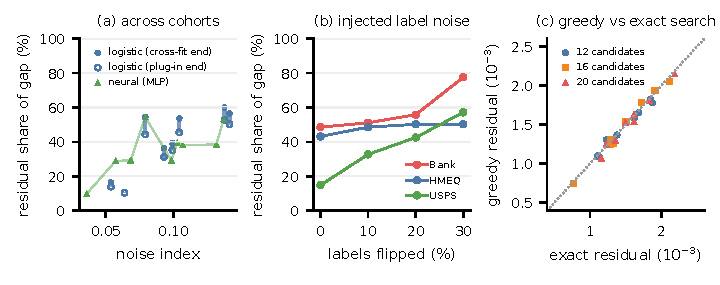
\includegraphics[width=\linewidth]{figures/fig_predict.pdf}
 \caption{(a) Residual share of the benchmark oracle gap against the label-noise index, one point per cohort; logistic learner with the plug-in (open) to cross-fitted (filled) bracket, and the neural learner (Table~\ref{tab:gradient}). (b) The same share when training labels are flipped at random within a cohort; 16 states per dose. (c) Residual under greedy search against exact search over all feasible sets in pools of 12, 16 and 20 candidates, 24 states per cohort and pool; dotted: identity.}
 \label{fig:predict}
\end{figure}

\paragraph{Budget and history.} Raising the budget target from 3 to 6 to 12 low-risk labels raised the family floor monotonically in all eight cohorts (paired increase from $k=3$ to $12$: $0.74$ $[0.67,0.82]$), because more labels were acquired, not riskier ones; per-label outcome variance of the chosen sets barely changes. A longer labeled history shrinks every part of the gap: from 68 to 512 historical labels the reported gap falls by a factor of 11--19, and the reuse share rises from 5--24\% to 22--68\%. The residual share keeps its ordering by noise at 128, 256 and 512 historical labels (Spearman $0.86$, $0.93$, $0.86$).

% ======================================================================
\section{What Changes for a Benchmark}
\label{sec:bench}
Pool-based benchmarks compare a strategy's learning curve with the oracle's. To see whether the decomposition changes such a comparison, we reproduced a benchmark step without delay or risk: the pending records are labeled and join the history, the budget is six labels from 24 candidates (Section~\ref{sec:setting}), and states are taken at four positions of the learning curve, with 68, 128, 256 and 512 historical labels. We used five cohorts with the logistic learner and six with the neural learner, including raw-pixel USPS as in CDALBench~\cite{werner2024cdalbench}, 32 states per cohort and position, and six practical strategies. For each strategy we compare two shortfalls: as a benchmark reports it, the oracle's gain minus the strategy's gain, both scored on $T_1$, where the oracle selected; and with reuse and luck removed, the cross-fitted ex-ante oracle's gain minus the strategy's gain, both scored on the held-out half $T_2$.

\begin{figure}[t]
 \centering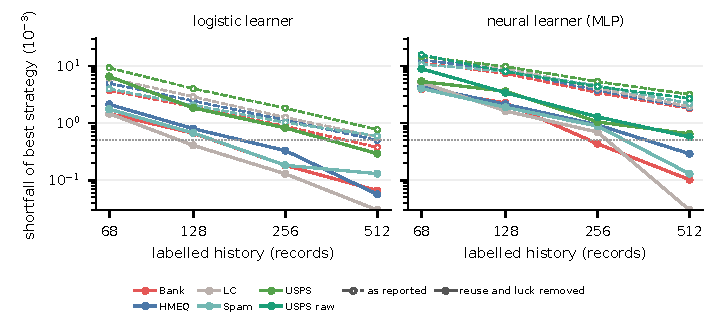
\includegraphics[width=\linewidth]{figures/fig_bench.pdf}
 \caption{Benchmark-style pool-based step (budget of six labels from 24 candidates, no delay). Shortfall of the best practical strategy behind the oracle along the learning curve, as reported (oracle and strategy scored on the evaluation half used for selection; dashed) and with reuse and luck removed (cross-fitted ex-ante oracle, held-out half; solid). The best strategy is chosen per cohort and position (descriptive). Dotted: material threshold. Log scale; values below $0.03$ are drawn at $0.03$.}
 \label{fig:bench}
\end{figure}

\paragraph{Early in the curve the conclusion holds; later it does not.} As reported, every strategy falls materially short of the oracle in every cohort at 68, 128 and 256 historical labels with both learners (pointwise 95\% intervals; 30 of 30 and 36 of 36 cohort--strategy pairs), and with the neural learner also at 512 (Fig.~\ref{fig:bench}). With reuse and luck removed, the shortfall of the best strategy falls by 30--76\% at the first position and is material for 30 of 30 and 36 of 36 pairs; at 128 labels for 14 of 30 and 35 of 36; at 256 labels for 2 of 30 and 13 of 36; and at 512 labels for none. With the neural learner at 512 labels, the reported shortfall of the best strategy is $1.8$--$3.2$ and the corrected one is $-0.03$ to $0.65$. Most of the difference late in the curve is test reuse, which makes up 64--80\% of the reported gap at 512 labels with the neural learner (37--70\% with the logistic learner); the residual makes up 2--19\% (8--40\%).

\paragraph{The registered prediction was only partly borne out.} At the first position we had predicted that, in the two noisiest cohorts, at least one strategy would no longer fall materially short once reuse and luck were removed, under the simultaneous intervals of the registered family. This happened in one of the two cohorts with each learner (LendingClub with the logistic learner, HMEQ with the neural learner), and also in Bank Marketing and Spambase, which we had not predicted; with the neural learner on raw-pixel USPS, as predicted, every strategy still falls materially short. The ranking of strategies by reported gain and by held-out gain disagreed on the top two in at least one cell for each learner. The benchmark conclusion that strategies fall short of the oracle is therefore sound at small labeled sets and on near-deterministic labels, and an artifact of evaluation later in the curve.

% ======================================================================
\section{Case Study: Risk-Constrained Acquisition}
\label{sec:replay}
\paragraph{Who closes the deployable part depends on the learner.} On real-label states under the risk budget, proxies derived from the logistic model close a large share of the cross-fitted gain where it is largest when the learner is logistic: on engineered HMEQ and LendingClub, TargetVar-greedy and Proxy-argmax capture $1.5$--$2.1$ of $3.2$--$3.4$. With the boosting learner the deployable part is still $0.7$--$2.7$, but no strategy captures more than $0.65$, and DC-PRISM's selection gap is material in six of eight credit cells. An information proxy helps only when it describes the learner that will be trained. In controlled worlds built around directional pending information, 83\% of hindsight headroom is ex-ante value; DC-PRISM gains $12.2$ $[7.6,16.8]$ over Safe-MinRisk with $3.1$ instead of 6 labels, most of it from the proxy evaluated over an anchored family (Proxy-argmax alone: $13.1$ $[6.1,20.2]$), while the conservative layer adds an unconfirmed $3.0$ $[-0.2,6.2]$.

\paragraph{Delayed replay.} To check whether single-round diagnoses predict multi-round outcomes, we replayed ten rounds with delayed labels (exploration labels after one round, ordinary labels after two; ALC-Brier averages ten round-start scores) with 512 fresh seeds per credit cell and 256 per readmission stream. Labels of candidates not acquired are used only for evaluation, so this is a full-label retrospective simulation, not a causal evaluation under selective labels. Table~\ref{tab:replay} matches the single-round diagnosis. Where information-greedy rules captured the deployable part and DC-PRISM did not (engineered HMEQ and LendingClub), DC-PRISM is materially worse than Fisher-cost, BAIT-greedy and TargetVar-greedy, by $2.5$--$3.8$; where its single-round gain over the reference was significant, it beats Safe-MinRisk and fixed count by $2.2$--$3.1$; where the protocol found little deployable value (natural streams, engineered UCI), no comparison is material. Realized adverse exposure exceeded the envelope in at most 4 of 40{,}960 acquisition rounds per credit policy and in none of 5{,}120 for readmission.

\begin{table}[t]
\caption{Delayed replay: comparator minus DC-PRISM ALC-Brier ($\times10^{-3}$; positive favors DC-PRISM; bold: material under the registered family).}
\label{tab:replay}
\centering\scriptsize
\setlength{\tabcolsep}{2.4pt}
\begin{tabular}{lrrrrrrrrrr}
\toprule
& \multicolumn{4}{c}{Credit, engineered} & \multicolumn{4}{c}{Credit, natural} & \multicolumn{2}{c}{Readmission} \\
\cmidrule(lr){2-5}\cmidrule(lr){6-9}\cmidrule(lr){10-11}
Comparator & HMEQ & LC & PPDai & UCI & HMEQ & LC & PPDai & UCI & eng. & nat. \\
\midrule
Safe-MinRisk & \textbf{2.4} & 0.4 & \textbf{3.1} & $-$0.1 & 0.2 & 0.2 & 0.4 & 0.1 & 0.0 & 0.2 \\
Fixed count & \textbf{2.2} & 0.4 & \textbf{2.4} & $-$0.1 & 0.1 & 0.1 & 0.3 & 0.0 & 0.4 & 0.2 \\
Random & 0.6 & $-$0.3 & \textbf{2.4} & 0.0 & 0.3 & 0.5 & 0.6 & 0.4 & 0.8 & 0.5 \\
Uncertainty & 0.5 & 1.4 & 0.7 & 0.0 & 0.4 & 0.4 & 0.1 & 0.1 & 0.4 & 0.0 \\
Fisher-cost & \textbf{$-$3.8} & \textbf{$-$3.3} & 0.8 & $-$0.1 & $-$0.3 & $-$0.1 & 0.1 & $-$0.1 & 1.0 & 0.0 \\
BAIT-greedy & \textbf{$-$3.6} & \textbf{$-$2.7} & 0.3 & 0.1 & $-$0.2 & 0.0 & 0.1 & 0.0 & \textbf{1.3} & 0.1 \\
TargetVar-greedy & \textbf{$-$3.5} & \textbf{$-$2.5} & 0.0 & 0.0 & $-$0.2 & $-$0.1 & 0.0 & $-$0.1 & \textbf{1.4} & 0.0 \\
\bottomrule
\end{tabular}
\end{table}

% ======================================================================
\section{Related Work}
\label{sec:related}
\paragraph{Evaluating active learning.} Active-learning gains are fragile under realistic evaluation~\cite{luth2023navigating}, sensitive to uncontrolled randomness~\cite{ji2023randomness} and inconsistent across domains~\cite{werner2023comparable,werner2024cdalbench}. Oracles are used to bound attainable performance~\cite{werner2024cdalbench,huseljic2026boss}, and Werner et al.\ observe that their greedy oracle overfits the test set~\cite{werner2023comparable}. We quantify that reuse along the learning curve, identify a second, aleatoric component that remains after the test set is split, and show that together they change a benchmark conclusion.

\paragraph{Regret, information value and uncertainty.} Ex-ante and ex-post regret are distinguished in decision-focused learning and robust optimization~\cite{schutte2023robust}; in bandits expected regret exceeds pseudo-regret by a noise term~\cite{bubeck2012regret,audibert2010regret}. The value of perfect information is classical~\cite{howard1966information,raiffa1961applied}, and selecting the best of noisy estimates is optimistic~\cite{smith2006optimizer,cawley2010overfitting}. Proper scoring rules such as the Brier score allow aleatoric and epistemic uncertainty to be separated~\cite{hofman2024quantifying}. Our contribution is not a new concept but a validated way to measure these terms for label-acquisition oracles on real data.

\paragraph{Acquisition under risk and delay.} Acquisition criteria range from uncertainty and transductive design to Fisher information, mutual and predictive information and decision loss~\cite{cohn1996active,settles2009active,lewis1994sequential,yu2006transductive,ash2021fishing,kirsch2019batchbald,bickfordsmith2023prediction,huang2026loss,chaloner1995bayesian}; budgets and knapsack constraints are handled by greedy selection~\cite{krause2005near,sviridenko2004note,tomanek2010cost}. Selective labels~\cite{lakkaraju2017selective,wei2021selective,kilbertus2020fair,keswani2024partial,crook2004reject}, safe exploration and safe active learning~\cite{sui2015safe,schreiter2015safe,wu2016conservative} and delayed feedback~\cite{joulani2013delayed,chapelle2014delayed,pham2022latency} motivate the risk-constrained setting of our case study.

% ======================================================================
\section{Conclusion}
\label{sec:conclusion}
An oracle that chooses labels after seeing them gains from three sources: reusing the evaluation set, outcome luck in the acquired labels, and genuine ex-ante information. Only the last is headroom. On labels that record random outcomes, such as repayment, readmission or subscription, luck and reuse made up most of the benchmark oracle's lead in our studies; on near-deterministic labels such as digits, most of the lead was real. Luck's share rose with label noise across cohorts and under injected noise, and reuse came to dominate later in the learning curve, where the conclusion that practical strategies fall short of the oracle no longer held once both were removed. We recommend that oracle comparisons report the held-out oracle gap, the residual at both ends of the bracket, the noise level of the labels and the sensitivity of the residual to the outcome model. A strategy should be judged against the part of the gap that remains.

\paragraph{Limitations.} The outcome model $\hat p$ does not identify the true conditional law, and our estimates condition on a fixed test set; the residual is most sensitive to the spread of $\hat p$, and single-cohort shares move by up to 25 points across reasonable models even though the noise ordering does not. The residual equals the family floor only approximately; exhaustive search was checked in pools of up to 20 candidates. Label flips are a controlled intervention, not a model of natural uncertainty. The benchmark-style study takes single steps at four positions rather than full trajectories, and pools, learners and budgets are modest; we did not study large pretrained models or multi-class labels. The risk envelope has its probabilistic meaning only under conditional independence and valid upper risk scores, which our empirical scores do not guarantee. The baselines are adaptations of their original criteria to the risk budget.

\bibliographystyle{splncs04}
\bibliography{refs}
\end{document}
